\section{Quantisatie}
\label{sec:quantisatie}

Tot nu toe hebben we altijd gewerkt met 32-bit floating-point getallen, wat voor onze doeleinden genoeg rekenprecisie geeft. Wanneer we deze getallen echter willen opslaan, zouden we ze liefst compacter willen voorstellen. Dit gaan we doen door te quantiseren: hierbij ronden we elke waarde af naar de dichtsbijzijnde waarde uit een beperkte verzameling die we zelf defini\"eren. Deze afronding zal de uiteindelijke fout op het eindresultaat verhogen, maar door deze verzamelingen goed te kiezen zullen we proberen een optimale afweging tussen de compressiefout en -factor te bekomen.\\

Wanneer we in deze sectie spreken over ``quantiseren naar $b$ bits'', doen we dit door de originele waarden te verschuiven en te schalen met specifieke waarden (die mee opgeslagen worden als 32-bit floats), zodat het nieuwe bereik exact overeenkomt met $[0, 2^b - 1]$. Hierna bekomen we de gequantiseerde waarden door alle waarden af te ronden naar het dichtsbijzijnde gehele getal. Dit is niet de enige mogelijke transformatie, maar we zullen ons in deze tekst hiertoe beperken. Verder zullen we de compressiefactor meten door telkens te quantiseren naar een verzameling met grootte gelijk aan $2^b$ (niet zozeer altijd met dezelfde $b$), waarna de geheugenruimte van per waarde geteld wordt als $b$ bits. 

\subsection{Kerntensor}

We zullen pas in de volgende subsectie quantisatietechnieken voor de factormatrices bespreken, maar zullen toch voor de komende experimenten moeten kiezen hoe deze verwerkt worden om de fout op het eindresultaat te berekenen. Zoals we in de vorige sectie zagen, wordt er quasi geen fout toegevoegd door de factormatrices te quantiseren naar 16 bits (en $\tau$ niet te quantiseren), dus we zullen dit ook doen voor de rest van de deze subsectie.

\subsubsection{Structuur van de kerntensor}

We weten dat gedurende de ST-HOSVD, bij het berekenen van de co\"ordinaten in de nieuwe basis, de eerste basisvectoren belangrijker zijn. Hierdoor zullen de absolute waarden van de eerste co\"ordinaten typisch ook groter zijn. Door dit proces meerdere malen toe te passen terwijl men over de modes itereert, zal men in feite de ``energie'' van de tensor concentreren in de posities met lage indices. De waarden in de uiteindelijke kerntensor zullen dus niet uniform verdeeld zijn.\\

Om hiermee rekening te houden zullen we in de rest van deze subsectie werken met ``lagen''. Met laag $i$ van een tensor bedoelen we de verzameling van posities met alle indices kleiner dan of gelijk aan $i$ en minstens \'e\'en index gelijk aan $i$ (denk aan schillen). In figuur \ref{fig:core-tensor-layers} wordt dit ge\"illustreerd. In de praktijk is de ongelijkheid tussen de lagen erg groot (zie figuur \ref{fig:core-tensor-values-distribution}, let op de logaritmische schaal).\\

\begin{figure}[H]
  \centering
  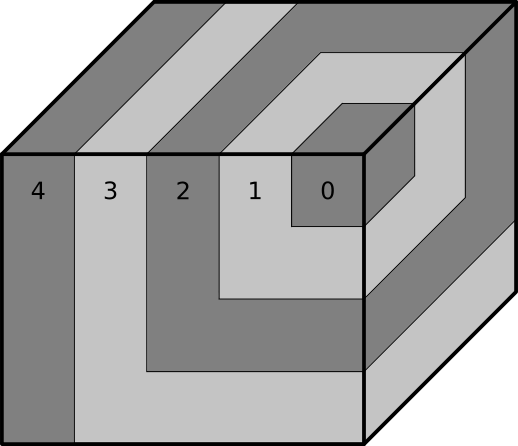
\includegraphics[scale=0.7]{images/core_tensor_layers.png}
  \caption{Lagen 0, \dots, 4 in een $5 \times 4 \times 3$ tensor.}
\label{fig:core-tensor-layers}
\end{figure}
\begin{figure}[H]
  \centering
  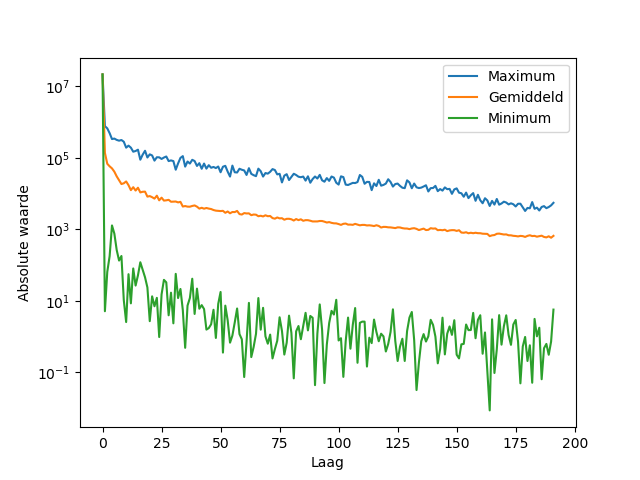
\includegraphics[scale=0.7]{images/core_tensor_values_distribution.png}
  \caption{Verdeling van absolute waarden in kerntensor bij Cuprite met relatieve doelfout 0.025.}
\label{fig:core-tensor-values-distribution}
\end{figure}

\newpage
Aangezien de meeste informatie in de eerste lagen zit, zullen we deze ongequantiseerd opslaan als 32-bit floats. Figuur \ref{fig:core-tensor-unquantized-portion} toont het effect van het aantal ongequantiseerde lagen bij vari\"erende aantallen quantisatiebits. Als quantisatietechniek gebruiken we simpelweg globale quantisatie: alle waarden buiten de eerste lagen worden gequantiseerd met hetzelfde aantal bits. Men ziet dat al een klein aantal lagen niet quantiseren een groot effect heeft op de fout met een insignificant effect op de compressiefactor. We kiezen ervoor om in het algemeen het aantal ongequantiseerde lagen zo te kiezen dat de norm van deze waarden minstens gelijk is aan 99.5\% van de norm van de tensor, wat bij Cuprite met relatieve doelfout 0.025 neerkomt op slechts 2 lagen.

\begin{figure}[H]
  \centering
  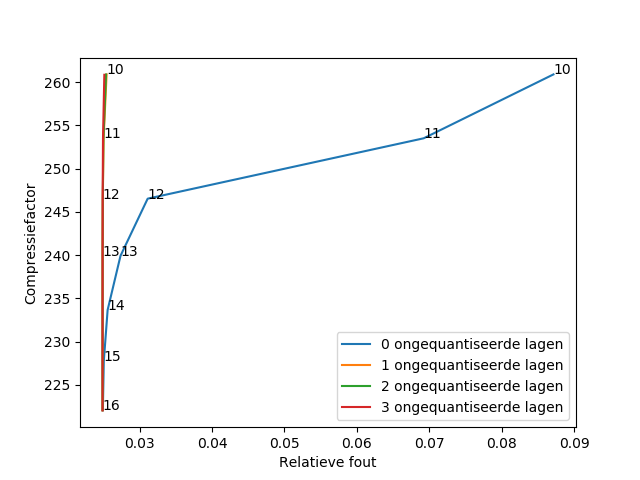
\includegraphics[scale=0.7]{images/core_tensor_unquantized_portion.png}
  \caption{Relatieve fout versus compressiefactor bij Cuprite met relatieve doelfout 0.025. De labels geven het aantal quantisatiebits aan.}
\label{fig:core-tensor-unquantized-portion}
\end{figure}

\subsubsection{Gelaagde quantisatie met constant aantal bits}

Zoals we eerder in figuur \ref{fig:core-tensor-values-distribution} zagen, zijn de waarden binnen de kerntensor erg ongelijk verdeeld, zelfs na het wegfilteren van de eerste twee lagen. Het is dus erg verspillend om alle andere waarden te quantiseren met hetzelfde aantal bits en dezelfde quantisatiestap, want het bereik van de waarden zal gedomineerd worden door het bereik van de eerste lagen, terwijl de laatste lagen slechts een erg klein deel van dit spectrum gebruiken.\\

Om dit op te lossen kunnen we elke laag apart quantiseren met een vast aantal bits dat constant blijft over de hele tensor, waardoor het bereik mooi past voor elke laag. Hierbij moeten we wel metadata gaan opslaan per laag en aangezien deze groeit met de afmetingen van de tensor zullen we deze meetellen in het geheugengebruik. Echter, bij een effici\"ente implementatie komt dit slechts neer op 12 bytes per laag, dus de \textit{overhead} van deze techniek is erg beperkt.

\subsubsection{Gelaagde quantisatie met variabel aantal bits}

Door het aantal quantisatiebits constant te houden over verschillende lagen, zal de quantisatiestap fijner worden voor de latere lagen. We weten echter dat alle kolommen uit de factormatrices genormaliseerd zijn, dus een vaste absolute fout op een waarde in de kerntensor zal zich onafhankelijk van de positie van deze waarde vertalen naar ongeveer dezelfde fout op het eindresultaat. Het is dus logischer om de latere lagen te quantiseren met een even grote stap, waardoor we minder bits nodig hebben.\\

Bij deze techniek zullen we voor elke laag een nieuw aantal quantisatiebits kiezen. We minimaliseren dit aantal zodat de quantisatiestap voor deze laag onder een bepaalde maximale stapgrootte ligt. We zullen deze controleren door expliciet het aantal quantisatiebits voor de eerste ongequantiseerde laag (de bits-parameter) te kiezen en dan de resulterende quantisatiestap gebruiken als bovengrens voor de verdere lagen. Voor het opslaan van het gekozen aantal bits zullen we \'e\'en byte extra per laag tellen, maar dit heeft natuurlijk geen significant effect.

\begin{figure}[H]
  \centering
  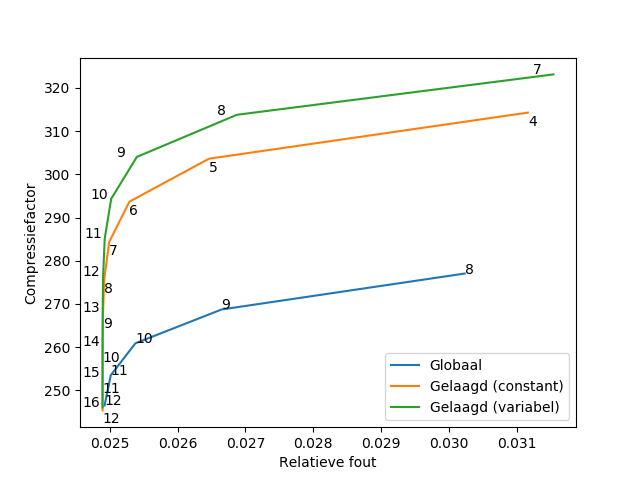
\includegraphics[scale=0.7]{images/core_tensor_quantization_comparison.png}
  \caption{Relatieve fout versus compressiefactor bij Cuprite met relatieve doelfout 0.025 en verschillende quantisatiemethoden voor de kerntensor. De labels geven de bits-parameterwaarden aan.}
\label{fig:core-tensor-quantization-comparison}
\end{figure}

\subsubsection{Besluit}

We hebben drie mogelijke quantisatietechnieken voor de kerntensor besproken: globale quantisatie en gelaagde quantisatie met een constant of variabel aantal bits. In figuur \ref{fig:core-tensor-quantization-comparison} zien we een experimentele vergelijking. Zoals verwacht comprimeert globale quantisatie het slechtste en kan men de gelaagde quantisatie verbeteren door te werken met een variabel aantal bits. Omwille van dit resultaat zullen we vanaf nu deze laatste techniek gebruiken (en specifiek voor de rest van deze sectie en sectie \ref{sec:encodering} met een bits-parameter van 12).

\subsection{Factormatrices}
\label{sec:quantisatie-factor-matrices}

Na de orthogonaliteitscompressie zal elke factormatrix voorgesteld worden als de combinatie van reflectoren en $\tau$-waarden (die samengevoegd worden tot \'e\'en $\tau$-vector per factormatrix). Zoals eerder besproken zullen we de $\tau$-vectoren niet quantiseren, omdat deze belangrijker zijn dan de andere waarden in de factormatrices en ons slechts 4 bytes per kolom per factormatrix kost. De waarden van de reflectoren nemen echter veel ruimte in en moeten best gequantiseerd worden.

\begin{figure}[H]
  \centering
  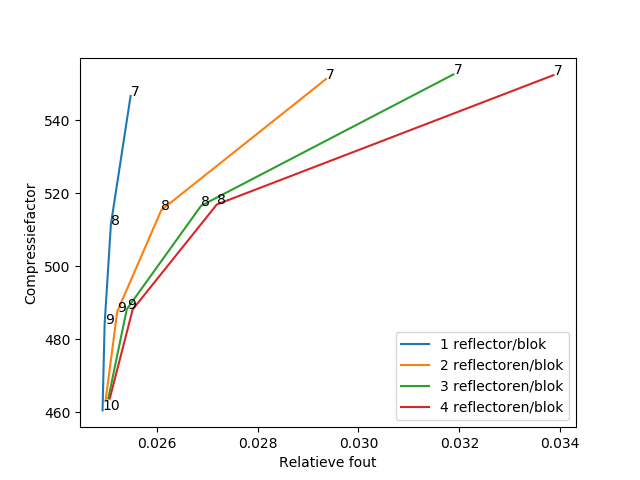
\includegraphics[scale=0.7]{images/factor_matrix_quantization_block_cols.png}
  \caption{Relatieve fout versus compressiefactor bij Cuprite met relatieve doelfout 0.025 en verschillende blokgroottes voor de quantisatie van de factormatrices. Quantisatie gebeurde gelaagd met norm-gebaseerde bit-aantal-selectie (zie vervolg subsectie). De labels geven de bits-parameterwaarden aan.}
\label{fig:factor-matrix-quantization-block-cols}
\end{figure}

Een eerste manier om dit te doen is weer met globale quantisatie per factormatrix (dus we berekenen \'e\'en specifiek bereik per matrix, niet voor alle matrices samen). We zagen echter al in de vorige subsectie dat het nuttig is om de waarden onder te verdelen in blokken, waardoor een specifieker bereik kan worden vastgelegd. Een gemiddelde reflector uit een factormatrix bevat echter veel minder waarden dan een gemiddelde laag uit de kerntensor, dus men zou kunnen proberen om meerdere reflectoren te groeperen per blok om zo de \textit{overhead} van de metadata (12 bytes per blok, eventueel 1 byte extra bij een variabel aantal bits) te beperken. Desalniettemin toont figuur \ref{fig:factor-matrix-quantization-block-cols} aan dat het beter is om dit niet te doen. We hebben ook ge\"experimenteerd met technieken om het aantal reflectoren per blok dynamisch te kiezen in functie van de dimensie van de reflector en het aantal quantisatiebits, maar dit gaf hetzelfde resultaat.\\

Om het aantal quantisatiebits te selecteren, kunnen we ook verschillende methoden gebruiken. De simpelste optie is om de bits-parameter te gebruiken als het constante aantal quantisatiebits voor elke reflector, maar hierbij houdt men geen rekening met enkele aspecten:

\begin{enumerate}

\item De eerste reflector be\"invloedt de reconstructie van alle kolommen van de factormatrix, de tweede reflector be\"invloedt alle kolommen buiten de eerste, ... Bijgevolg zijn de eerste reflectoren belangrijker en zou men deze met meer precisie kunnen bijhouden. Aangezien dit effect moeilijk te quantiseren valt houden we hier geen rekening mee.

\item De eerste singuliere vectoren zijn belangrijker dan de laatste, waardoor we beter meer precisie gebruiken voor deze. Bij ``norm-gebaseerde'' selectie zullen we het aantal bits per waarde binnen een reflector ongeveer proportioneel kiezen met het logaritme van de norm van de corresponderende snede uit de kerntensor (de waarden die later vermenigvuldigd zullen worden met corresponderende singuliere vector). De bits-parameter legt vast hoeveel quantisatiebits er voor de eerste reflector gekozen moeten worden.

\item De eerste reflectoren hebben een hogere dimensie en worden dus voorgesteld door meer waarden, waardoor het aantal bits per waarde hier misschien verlaagd moet worden. Bij ``norm- en dimensie-gebaseerde'' selectie zal het totaal aantal gebruikte bits per reflector ongeveer proportioneel zijn met de norm van de corresponderende snede uit de kerntensor. Zoals eerder wordt het aantal quantisatiebits per waarde voor de eerste reflector vastgelegd door de bits-parameter.

\end{enumerate}

In figuur \ref{fig:factor-matrix-quantization-comparison} vindt men een vergelijking van de besproken methoden. Zoals verwacht is gelaagde quantisatie opnieuw veel beter. Voor de bitselectie is de norm-gebaseerde techniek het beste, gevolgd door de norm- en dimensie-gebaseerde techniek en uiteindelijk constante selectie. Men zou dit kunnen verklaren door het effect van het eerste aspect dat we eerder bespraken (omzetting van reflectoren naar singuliere vectoren). Dit hebben we namelijk niet in rekening gebracht maar zou de norm-gebaseerde selectie moeten helpen. In ieder geval is dit de beste techniek en zal deze vanaf nu gebruikt worden. Voor de volgende sectie zullen we werken met een bits-parameter van 10, waardoor er geen merkbare fout toegevoegd zal worden.

\begin{figure}[H]
  \centering
  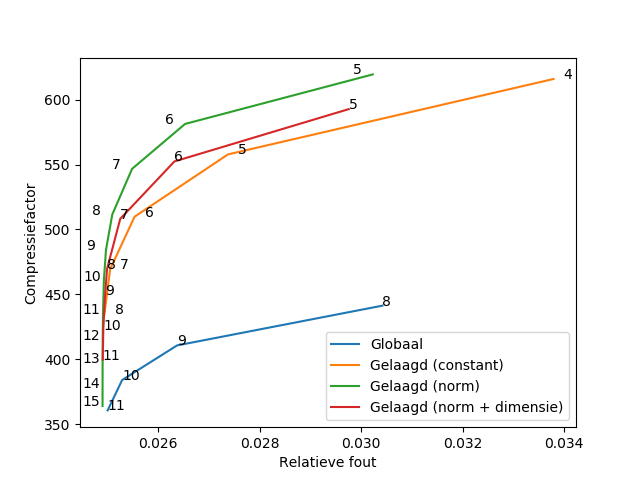
\includegraphics[scale=0.6]{images/factor_matrix_quantization_comparison.png}
  \caption{Relatieve fout versus compressiefactor bij Cuprite met relatieve doelfout 0.025. De labels geven de bits-parameterwaarden aan.}
\label{fig:factor-matrix-quantization-comparison}
\end{figure}